\chapter{Architettura CUDA}
\section{Cos'è CUDA}
CUDA ( Compute Unfied Device Architecture) è un architettura hardware creata da NVIDIA e pensata per l’elaborazione parallela che si basa dunque sulla suddivisione di un problema in sottoproblemi e lo svolgimento di ognuno di questi concorrentemente.
Tutto ciò è possibile sfruttando la potenza di calcolo della GPU (unità di elaborazione grafica) che assieme alla CPU permette di rendere molto efficiente in termini di tempo l’esecuzione di molte applicazioni.
Il calcolo parallelo su GPU offre prestazioni senza precedenti caricando porzioni \textbf{compute-intensive} dell'applicazione sulle GPU, mentre la porzione rimanente di codice continua ed eseguire su CPU. Pertanto, le GPU devono operare congiuntamente con le CPU mediante bus PCI-Express

\begin{figure}[H]
\centering
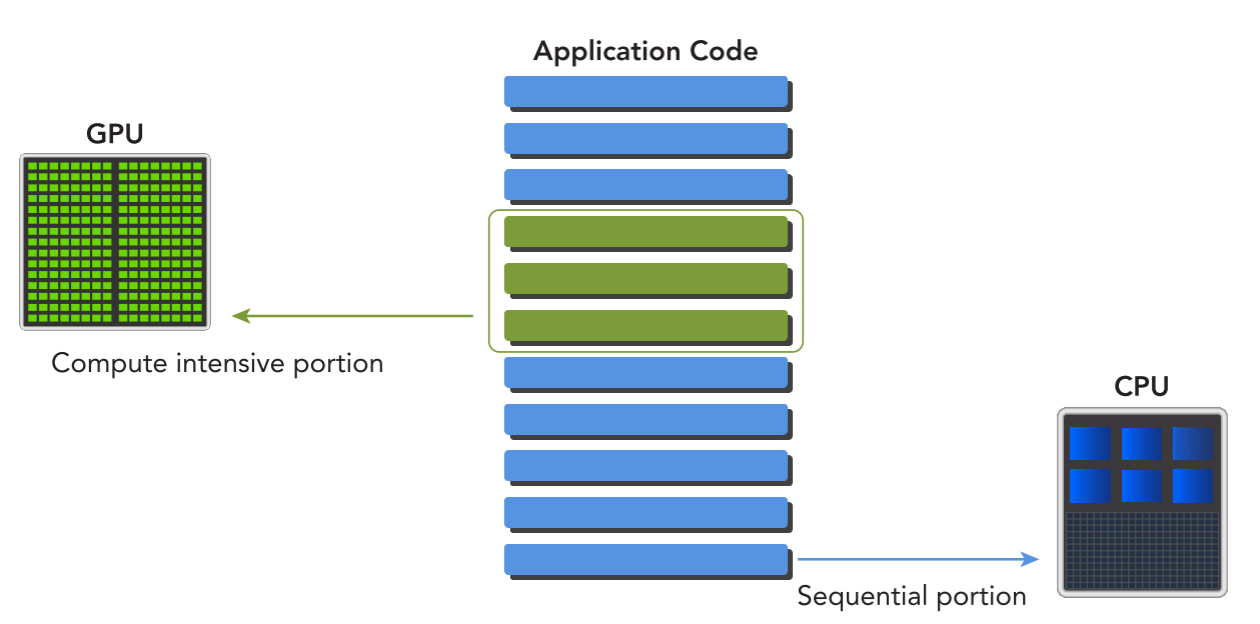
\includegraphics[scale=0.5]{img/cpu-gpu.png}
\caption{Divisione delle operazioni tra GPU e CPU in ambiente CUDA}
\end{figure}

\paragraph{}
Le applicazioni in cui CPU e GPU lavorano insieme consistono di due parti:
\begin{itemize}
\item codice Host
\item codice Device
\end{itemize}


Il codice Host esegue su \textbf{CPUs} e il codice device esegue su \textbf{GPUs}. Il codice CPU è responsabile della gestione dell'ambiente, dell'IO e della gestione dei dati per il device stesso, prima di caricare task intensivi sul device. La GPU è usata per accelerare l'esecuzione di questa porzione di codice basandosi sul parallelismo dei dati. La CPU è ottimizzata per sequenze di operazioni in cui il controllo del flusso è impredicibile; le GPU lo sono per carichi dominati da semplice flusso di controllo.

\begin{figure}[H]
\centering
\includegraphics[scale=0.6]{img/Performancecpu-gpu.png}
\caption{Prestazioni tra GPU e CPU in relazione a grado di parallelismo e quantità dei dati da elaborare.}
\end{figure}

\section{Il modello di programmazione CUDA}
CUDA come tutti i modelli di programmazione fornisce un’ \textbf{astrazione} della macchina e si  pone come ponte tra il software e l’hardware. Il programma, scritto seguendo il modello di programmazione, definisce come condividere le informazione e coordinare le attività mentre fornisce una visione logica del computer attraverso strumenti come il compilatore, le librerie, sistema operativo e primitive hardware.


\begin{figure}[H]
\centering
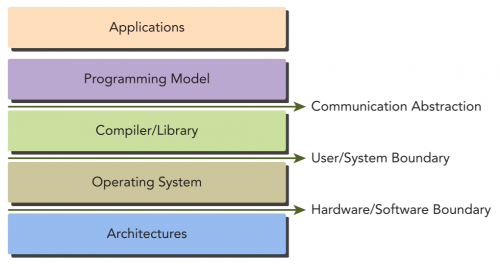
\includegraphics[scale=0.6]{img/modello.png}
\caption{Prestazioni tra GPU e CPU in relazione a grado di parallelismo e quantità dei dati da elaborare.}
\end{figure}

In particolare il modello CUDA offre una visione dell’architettura GPU per sfruttarne a pieno la potenza di calcolo:
\begin{itemize}
\item Struttura gerarchica dell’organizzazione dei Threads
\item Struttura gerarchica dell’organizzazione della memoria
\end{itemize}

\subsection{Struttura di un programma CUDA}
La struttura di un programma CUDA evidenzia la coesistenza di un host (CPU) e \textbf{uno o più} devices (GPU). Le funzioni che devono essere eseguite dal device sono integrate nel sorgente C e indicano al device quali operazioni effettuare, su quali dati e con quale grado di parallelismo svolgerle. Il modello CUDA quindi permette l’esecuzione di applicazioni su modelli di calcolo \textbf{eterogenei} (CPU + GPU) semplicemente annotando il codice con un piccolo insieme di estensioni del linguaggio C separando:
\begin{itemize}
\item \textit{HOST}: CPU+ Memoria (\textbf{Host} memory)
\item \textit{DEVICE}: GPU + Memoria (\textbf{Device} memory)
\end{itemize}

\subsubsection{Kernel}
Il codice eseguito sul device è chiamato kernel ed è, come detto, denotato da opportune keyword CUDA. Di fatto si tratta di una procedura sequenziale che CUDA gestisce in modo concorrente mediante lo scheduling dei thread sui vari core. Il modello CUDA è \textbf{asincrono} permettendo così che le computazioni su GPU e CPU siano sovrapponibili e gestite da comunicazioni host-device

\begin{figure}[H]
\centering
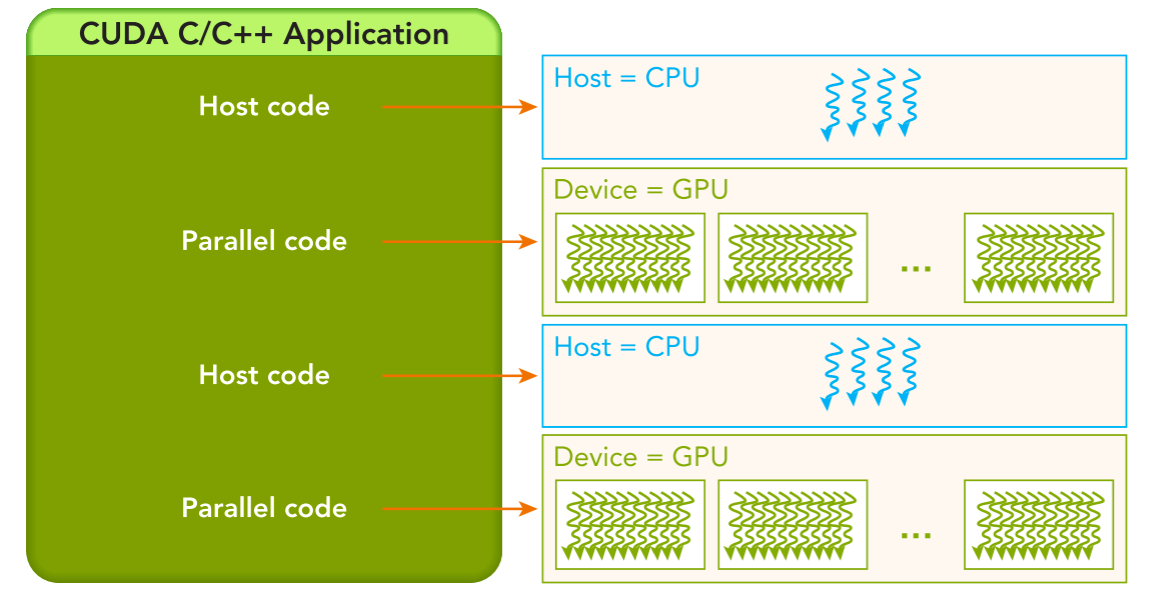
\includegraphics[scale=0.6]{img/program.png}
\caption{Prestazioni tra GPU e CPU in relazione a grado di parallelismo e quantità dei dati da elaborare.}
\end{figure}

\subsection{Flusso tipico}
Il tipico flusso di un programma CUDA è composto di tre fasi:
\begin{itemize}
\item Copia dei dati dalla CPU memory alla GPU memory
\item Invocazione dei kernel per operare su dati memorizzati in GPU memory
\item Copa dei dati dalla GPU memory alla CPU memory

\end{itemize}



Il codice per il device viene compilato a runtime dal compilatore NVCC mentre il codice C/C++ dal compilatore C ed eseguito su CPU. Quando un kernel viene lanciato, viene eseguito da un elevato numero di thread, suddivisi in blocchi che collettivamente vengono chiamati \textbf{griglia}.


\begin{figure}[H]
\centering
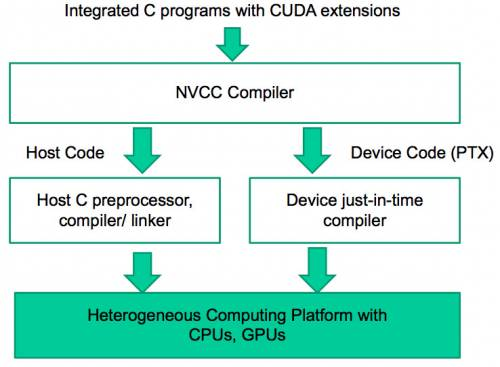
\includegraphics[scale=0.6]{img/nvcc}
\caption{Prestazioni tra GPU e CPU in relazione a grado di parallelismo e quantità dei dati da elaborare.}
\end{figure}

